\section{Deep Parameter Optimisation}
\label{sec_deep_parameter_optimisation}

Figure \ref{system} shows the overall work flow of the deep parameter optimisation. The approach takes the source code of the program under tuning, a set of test data and a set of non-functional properties of interests as inputs. 
It first applies mutation analysis and a non-dominated rank algorithm to discover potential locations for deep parameters, explained in Section \ref{discovering}. It then promotes deep parameters based on the type of expressions found at the locations, explained in Section \ref{exposing}. Finally, to tune the program, a search-based algorithm is used to search for optimised values for both shallow and deep parameters, explained in Section \ref{sec_nsgaii}.

\begin{figure*}[htbp]
\centering
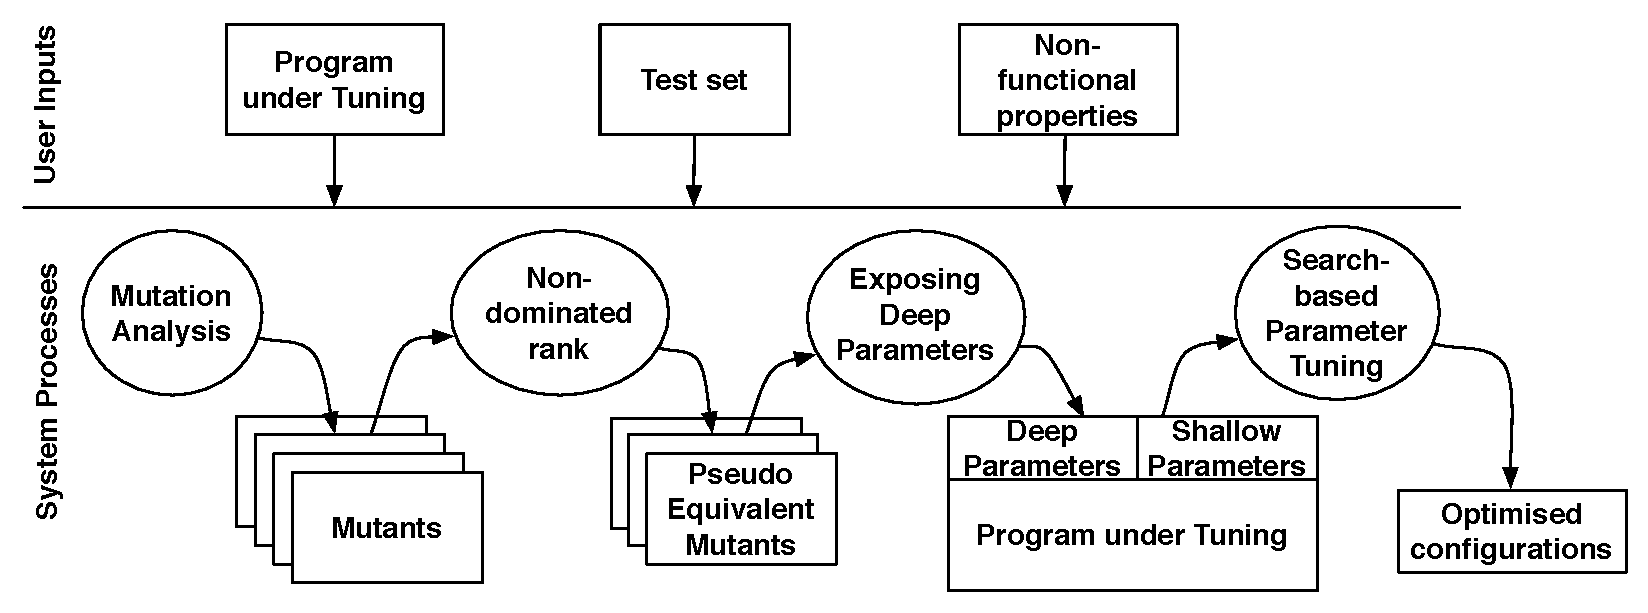
\includegraphics[width=6.2in]{pics/new_system}
\caption{Deep parameter optimisation workflow}\label{system}
\end{figure*}

\subsection{Discovering locations for deep parameters}
\label{discovering}
The first step is to identify potential locations at which we could expose deep parameters. 
In our approach, we represent the input program as an abstract syntax tree and a potential location $L$ is an expression node of the AST. 
We want to find a set of locations $L_D$ such that when we tune the value of the expression at $L_D$, some non-functional properties of the program could be improved while the program remains the same functional behaviour. 
%We use software testing to valid the functional behaviour of the program. 
To valid the functional behaviour of the tuned program, we test the tuned program with the input test set and compare the output with the test output of the original program.

We use mutation analysis to automate the process of searching for locations $L_D$. Mutant analysis deliberately makes simple syntactic changes to the input program, to create a set of various version programs called mutants, each contains a different syntactic change. A transformation rule that generates a mutant from the input program is known as a mutation operator. By carefully choosing mutation operators, we can use mutants to simulate the effect of making changes at all potential location $L$ . Table \ref{tab:cmop} shows the operators we used to generate mutants, covering locations of a constants, relational, logical and arithmetic expressions. 
To assess the quality of a mutant, we test each mutant against the input test set and record the values of the non-functional properties. If the result of running a mutant is different from the result of running the origianl program for any test data in the input test set, then the mutant is said to be ``killed'', otherwise it is said to have ``survived''. 

\begin{table} [htbp]
\caption{Selected mutation operators}
\label{tab:cmop} 
\begin{center}
\begin{tabular}{ | c | l |}
  \hline
  Mutation Operators & Description \\ 
\hline
  CRCR & Required constant replacement \\
  OAAN & Arithmetic operator mutation \\
  OAAA & Arithmetic assignment mutation \\
  OCNG & Logical context negation \\
  OIDO & Increment/decrement mutation  \\
  OLLN & Logical operator mutation  \\ 
  OLNG & Logical negation \\
  ORRN & Relational operator mutation \\
  OBBA & Bitwise assignment mutation \\
  OBBN & Bitwise operator mutation \\
\hline
\end{tabular} 
\end{center} 
\end{table} 

After all mutants are executed, we first filter out the killed mutants which fail to hold the functional behaviour.  Thus we only select pseudo equivalent mutants which preserve the behavious of the original program. 
In practice, there are a large number of equivalent mutants \cite{5477100} generated and we only want to select a subset from them which represents the locations that could have the greatest impact on the non-functional properties of interests.  
We achieve this by ranking the mutants based on their non-functional properties using the non-dominated sorting approach in the NSGAII algorithm \cite{996017}. Each mutant is assigned with a Pareto Level value and a Crowd Distance value, where Pareto Level $n$ means a mutant will be on the Pareto Front after all the mutants with Pareto Level less than $n$ are removed, while Crowd Distance indicates how close a mutant is to its neighbours on the same Pareto Level. Then a mutant is better than another in terms of non-dominated sorting if its Pareto Level is smaller or their Pareto Level is the same but the former is less crowded (bigger Crowd Distance) than the latter. After sorting all the mutants in terms of their non-functional properties, we apply a greedy algorithm to pick the first $k$ locations that could best influence the non-functional properties of the original, where $k$ is the desired number of Deep Parameters one wants to expose.

\subsection{Exposing deep parameters}
\label{exposing}
The second step is to expose deep parameters which allow users to modify the value of the expression at selected locations. Based on the type of mutation, we first classify the selected mutants into two sets. $Set\ 1$ contains mutants generated from CRCR, OAAN, OAAA and OIDO operators, which simulate locations with non-logical expressions. $Set\ 2$ constrains mutants generated from the OCNG, OLLN, OLNG and ORRN operators, which simulate locations with logical expressions. 
Given an location $L$, $E_L$ is the expression at the location $L$, we use the following transformation rules to rewrite $E_L$ with a new parameter $v$.

\begin{equation}
 E_L \rightarrow \left\{
  \begin{array}{l l}
    (E_L + v) & \quad \text{if $L$ $\in$ Set 1}\\
    (E_L) \ xor \ v & \quad \text{if $L$ $\in$ Set 2}
    \end{array} \right.
\end{equation}

We use addition to affect the value of non-logical expression and exclusive or to affect the logical ones.
Finally we expose $v$ as a `public' parameter so that users can assign value to $v$ through parameter passing or APIs.

\subsection{Search-based parameter tuning}
\label{sec_nsgaii}

Although the exposed deep parameters can provide additional `knobs' to turn the program, but they cannot completely substitute the shallow parameters of the program.  Thus, in this work, we propose to use both shallow parameters and deep parameters and tune them together with SBSE \cite{Harman:2007:CSF:1253532.1254729}. Because we are interested in multiple non-functional properties, a multi-objective Genetic Algorithm, NSGA II\cite{996017}, is applied on the searching of optimal values for both shallow and deep parameters.


We use an integer vector to represent the list of parameters under tuning. Each gene stores a solution value for one parameter. At each generation, our NSGAII first applies tournament selection followed by a scattered crossover and uniform mutation operation. In this work our fitness functions are designed to capture two non-functional properties: execution time and memory consumption. To measure execution time, \emph{Glibc}'s \emph{wait4} system call is used to calculate the total cpu time consumed by the program. For memory consumption, we instrumented the program under tuning to record the high-water mark of the virtual memory consumption. This is due to the fact that the physical memory reported by OS is not always deterministic. After fitness evaluation, a standard NSGA II non-dominated selection is applied to create the next generation. Finally, all non-dominating solution in the last population are returned.
